\documentclass{article}
\usepackage{math}
\usepackage{tikz-cd}
\usepackage{tikz}
\usetikzlibrary {arrows.meta}

\title{An Introduction to Category Theory}
\author{Andrew L Jones}\date{}

\begin{document}
\maketitle

% INTRODUCTION

\section*{Introduction}
One of the most abstract fields of mathematics: Category Theory arose from the practice of representing mathematical structures as diagrams on blackboards. Although its origins might be in the corporeal world of chalkboards and erasers, Category Theory is a field of mathematics that emphasizes the abstract study of mathematics as form over the applied use of mathematics as calculation. As Lawvere states, it "has long been felt in advanced algebra and topology, namely that the substance of mathematics resides not in Substance (as it is made to seem when $\in$ is the irreducible predicate, with the accompanying necessity of defining all concepts in terms of a rigid elementhood relation) but in Form" \cite{Lawvere01}. 

In more concrete terms, chasing the underlying fundamental Substances that can establish a foundation for mathematics might not be as fruitful as studying the forms that mathematics can take on. These forms in turn can often reveal aspects of mathematics that get lost in the event horizon of constraints and predicates that mathematical foundations require. Category theory is a language that allows mathematicians to study mathematics as form.

% FIRST SECTION 

\section{Objects and Arrows}
Fundamental to this study of mathematical form is the concept of a Category.
\begin{definition}
A category consists of a collection of Objects $ob(c)$; a collection $mor(C)$ of Arrows; a collection of Objects to map from $dom(C)$; a collection of Objects to map to $cod(C)$. Categories must satisfy three conditions: \begin{enumerate}
    \item Arrows must be associative.
    \item Arrows most compose with other Arrows.
    \item All Objects must have a left and right identity that is part of the Arrows.
  \end{enumerate}
\end{definition}
\begin{example}
Construct a Category 2 with two Objects $A$ and $B$ and two identity arrows $id_A$ and $id_B$, and one arrow $f: A \mapsto B$. As composition is restricted to $id_B \circ f = f = f \circ id_A$ and associativity is vacuous. This yields the diagram:
\begin{center}
\begin{tikzcd}
\arrow[loop left]{l}{\mathrm{id}_A} \ar{r}A & B \arrow[loop right]{r}{\mathrm{id}_{B}}
\end{tikzcd}
\end{center}
\end{example}
\begin{remark}
Note that Category 2 is a Category by virtue of its form and not what the arrows and objects represent. This level of abstraction is the essence of Category Theory.
\end{remark}
\subsection{Small \& Discrete}
Despite this high level of abstraction, Categories are often used on real mathematical objects. Arrows can be and usually are functions. Objects can be and frequently are sets.
\begin{definition}
Categories in which every Object forms a set are called \textbf{small} categories.
\end{definition}
\begin{theorem}
The Group $(\mathbb{Z}, +)$ is a small category.
\end{theorem}
\begin{proof}
Construct a Category $Z$ with $ob(Z) = \{\mathbb{Z}\}$ and $mor(Z) \in \mathbb{Z}$. Hence, composition is given by the Group's binary operator $+$: $f \circ g = f + g$. $Id_Z = 0$ and $g + 0 = g = 0 + g$. Observe that $+$ is associative and therefore $Z$ is a small category.
\end{proof}
\begin{definition}
 Categories in which every arrow is $id$ are called \textbf{discrete} categories.
\end{definition}
\begin{theorem}
The Poset $(\mathbb{Z}, =)$ is a discrete category.
\end{theorem}
\begin{proof}
Construct a Category $D$ with $ob(D) = \{\mathbb{Z}\}$ and all $mor(D) = (z,z) \in \mathbb{Z}$. Compositions is given by the relation $=$ which implies all arrows must satisfy the constraint $z = z$. Associativity and composition are satisfied by the relation. Therefore $D$ is a discrete category.
\end{proof}
The categories given by the Group $(\mathbb{Z}, +)$ and the Poset $(\mathbb{Z}, =)$ satisfy the same laws of a category in different ways. As Emily Riehl puts it, "the action of packaging each variety of objects into a category shifts one's perspective from the particularities of each mathematical sub-discipline to the potential commonalities between them."\cite{Riehl01}. Equality and the addition of integers abstract into comparable forms.
\subsection{Comparing Forests}
The radical similarities of Categories is not limited to just linking operations and relations. To quote Herrlich and Strecker: "Category Theory involves the next level of abstraction-i.e., comparing forests." \cite{Herrlich01}. This abstraction goes so far that the actual value of the sets often matter less than the composition of arrows. As Milewski puts it: “Category theory is extreme in the sense that it actively discourages us from looking inside the objects. An object in category theory is an abstract nebulous entity.” \cite{Milewski01}. This level of abstraction shows up prominently in the convention of representing categories as diagrams.

\begin{center}
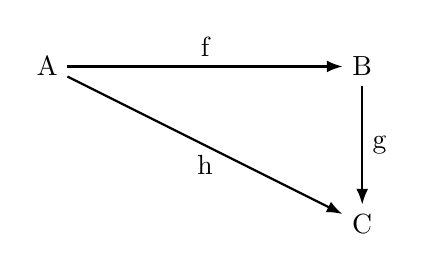
\begin{tikzpicture}
\path (-2,2) node (A) [black] {A};
\path (2,2) node (B) [black] {B};
\path (2,0) node (C) [black] {C};
\draw[thick, ->, -{Latex[length=2mm]}] (A) -- (B) node[midway,above] {f};
\draw[thick, ->, -{Latex[length=2mm]}] (B) -- (C) node[midway,right] {g};
\draw[thick, ->, -{Latex[length=2mm]}] (A) -- (C) node[midway,below] {h};
\end{tikzpicture}
\end{center}
The above diagram could represent a Poset, a Monoid, a Ring, or myriad other mathematical structures. As we have $f: A \to B$, $g: B\to C$, $h = g \circ f$ and following $f$ to $g$ has the same result as $h$, we can claim this diagram commutes.

\begin{definition}
    A diagram \textbf{commutes} when all parallel arrows obtained by composing arrows in the diagram agree.
\end{definition}
The reliance on diagrams is more than instructive in Category Theory. When a diagram commutes, we have graphically proven that collections of objects and arrows construct a category. This leads to a peculiar property of a Category.
\begin{corollary}
 For each Category $C$ there is an opposite category obtained by reversing all the arrows called $C^{op}$
\begin{center}
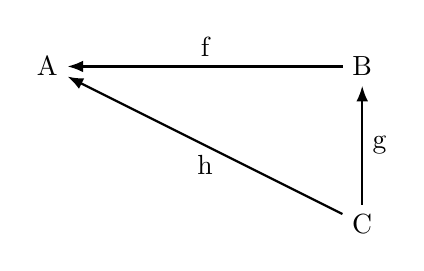
\begin{tikzpicture}
\path (-2,2) node (A) [black] {A};
\path (2,2) node (B) [black] {B};
\path (2,0) node (C) [black] {C};
\draw[thick, ->, -{Latex[length=2mm]}] (B) -- (A) node[midway,above] {f};
\draw[thick, ->, -{Latex[length=2mm]}] (C) -- (B) node[midway,right] {g};
\draw[thick, ->, -{Latex[length=2mm]}] (C) -- (A) node[midway,below] {h};
\end{tikzpicture}
\end{center}
As $f \circ g = h$ we can conclude the diagram commutes.
\end{corollary}

% SECOND SECTION

\section{Functors}
Categories commute by composition of arrows. Unsurprisingly, Category Theory contains many different types of Arrows. Functors are a type of Arrow that maps between Categories while preserving structure.
\begin{definition}
    Assume that $A$ and $B$ are categories. A Functor $F$ is a map between Categories such that:
    \begin{enumerate}
        \item Each Object from $A$ maps to an Object in $B$
        \item Each Arrow from $A$ maps to an Arrow in $B$ such that:
        \begin{enumerate}
            \item The identity arrows  $Id_A$ and $Id_B$ hold
            \item Preserves composition such that $F(f \circ g) = F(f)\circ F(g)$ where $f \in mor(A)$ and $g \in mor(B)$.
        \end{enumerate}
    \end{enumerate}
\end{definition}

\begin{theorem}
The function $F: x \mapsto |x|$ is a functor from $\mathbb{Z}$ to $\mathbb{Z_{\ge 0}}$
\end{theorem}
\begin{proof}
Fix $a,b \in \mathbb{R}$ and $f: x \mapsto ax$ and $g: x \mapsto bx$. Therefore $g \circ f = bax$. Hence, $F(g \circ f) = F(f) \circ F(g)$. Observe that $|bax| = |b|ax||$.
\end{proof}
\begin{center}
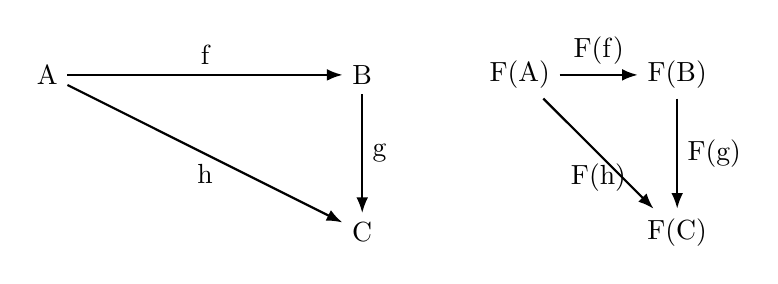
\begin{tikzpicture}
\usetikzlibrary {arrows.meta}
\path (-2,2) node (A) [black] {A};
\path (2,2) node (B) [black] {B};
\path (2,0) node (C) [black] {C};
\path (4,2) node (FA) [black] {F(A)};
\path (6,2) node (FB) [black] {F(B)};
\path (6,0) node (FC) [black] {F(C)};
\draw[thick, ->, -{Latex[length=2mm]}] (A) -- (B) node[midway,above] {f};
\draw[thick, ->, -{Latex[length=2mm]}] (B) -- (C) node[midway,right] {g};
\draw[thick, ->, -{Latex[length=2mm]}] (A) -- (C) node[midway,below] {h};
\draw[thick, ->, -{Latex[length=2mm]}] (FA) -- (FB) node[midway,above] {F(f)};
\draw[thick, ->, -{Latex[length=2mm]}] (FB) -- (FC) node[midway,right] {F(g)};
\draw[thick, ->, -{Latex[length=2mm]}] (FA) -- (FC) node[midway,below] {F(h)};
\end{tikzpicture}
\end{center}
Therefore the diagram commutes.

% BIBLIOGRAPHY

\bibliographystyle{plain}  % see:  https://www.overleaf.com/learn/latex/Bibtex_bibliography_styles
\bibliography{testbib}
\end{document}

